\section{B$^+$Tree}

\begin{definition}
  B$^+$Tree is a B-Tree where keys are stored exclusively in leaf nodes.
\end{definition}

Separator keys may not match to keys contained in leaf nodes and may be freely chosen, with the only requirement being they point to correct subtree during a search. Leaf nodes may optionally include a pointer to the right sibling.

\begin{figure}[H]
  \centering
  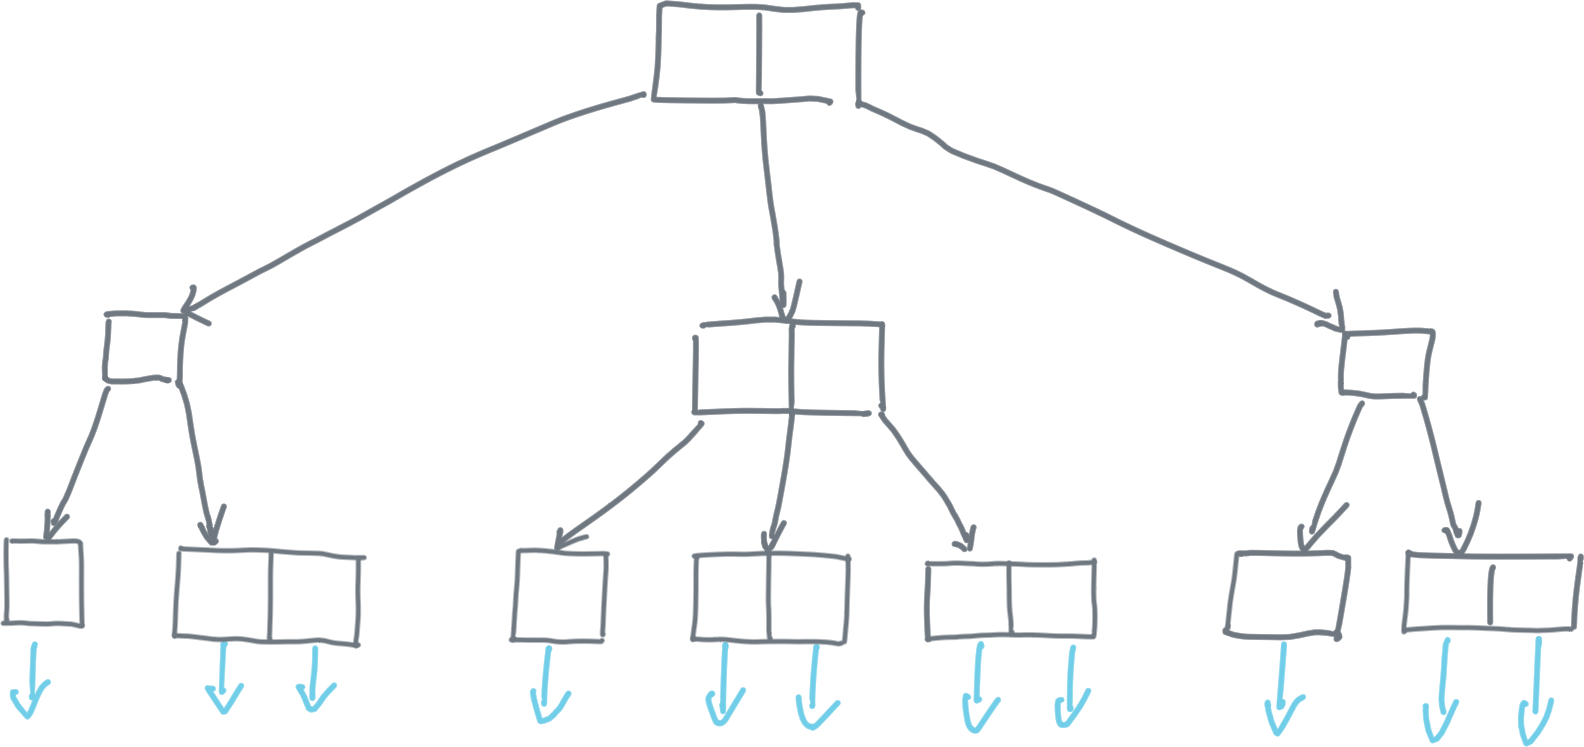
\includegraphics[width=\textwidth]{components/figure/b+tree.png}
  \caption{B+Tree with $Order$ = 3}
  \label{figure:b+tree}
\end{figure}

By storing keys in leaf nodes, the branching factor of internal nodes is maximized, which results in lower tree height and fewer I/O operations.

Deletion of a node in B$^+$Tree is also simplified, as we can directly traverse to the leaf nodes when searching for the key to delete. Tree rebalancing is still desired to preserve the invariants of B-Tree.

B$^+$Tree do trade increased space complexity for the ability of trivial sequential querying.